%%%%%%%%%%%%%%%%%%%%%%%%%%%%%%%%%%%%%%%%%%%%%%%%%%%%%%%%%%%%%%%%%%%%%%%%%%%%%
%% Descr:       Vorlage für Berichte der DHBW-Karlsruhe, Ein Kapitel
%% Author:      Prof. Dr. Jürgen Vollmer, vollmer@dhbw-karlsruhe.de
%% $Id: kapitel2.tex,v 1.5 2017/10/06 14:02:51 vollmer Exp $
%%  -*- coding: utf-8 -*-
%%%%%%%%%%%%%%%%%%%%%%%%%%%%%%%%%%%%%%%%%%%%%%%%%%%%%%%%%%%%%%%%%%%%%%%%%%%%%%%

\chapter{Konzeption}
\label{chap:Konzeption}
In diesem Kapitel wird das erarbeitete Konzept dieser Ausarbeitung dargelegt. Unter dessen die Überlegungen zu einzelnen 
Arbeitsschritten und dem grundsätzlich angedachten Aufbau des Projekts, sowie Entscheidungs- und Beweggründe wieso bestimmte 
Technologien gewählt wurden. Zu Beginn wird auf die Einsatzmöglichkeiten (\ref{chap:Arbeitsumgebung}), in der die Applikation Anwendung 
finden könnte, eingegangen. Anschließend werden die Grundgedanken zu den einzelnen Phasen, Scan-Phase (\ref{chap:Scan-Phase}) und 
Visualisierungs-Phase (\ref{chap:Visualisierungs-Phase}) des Systems erläutert, was sie beinhalten und wie sie funktionstechnisch 
angedacht sind. Mit den zugrundeliegenden Informationen wird auf das Architekturkonzept (\ref{chap:Architekturkonzept}), sowie auf das 
Softwarekonzept (\ref{chap:Architekturkonzept}) eingegangen. Des Weiteren werden die Hintergründe der Wahl des AR-Frameworks 
(\ref{chap:Auswahl des AR Frameworks}) aufgezeigt und abschließend wird noch das konzipierte und prototypische Datenmodell 
(\ref{chap:Datenmodell}) dargelegt.

\section{Arbeitsumgebung / Umfeld}
\label{chap:Arbeitsumgebung}

\section{Objekterkennung / Scan-Phase}
\label{chap:Scan-Phase}

\section{Visualisierungs-Phase}
\label{chap:Visualisierungs-Phase}

\section{Architekturkonzept}
\label{chap:Architekturkonzept}
Um das \acl{AR} basierte Assistenzsystem grundlegend zu definieren, ist es von Vorteil ein geeignetes Konzept sowie einen ersten Entwurf zu 
erstellen. Dieser sollte als Fundament für eine Applikation mit stetig steigender Anzahl an Funktionen dienen. Anfänglich soll der Prototyp 
dafür sorgen, einen Überblick über beispielsweise Maschinen in Produktionshallen zu verschaffen. Dies bedeutet, dass Informationen zu bestimmten 
Objekten schnell zur Verfügung stehen und eventuell defekte Maschinen zügig aufzufinden sind.  
\begin{figure}[hbt!]
    \centering
    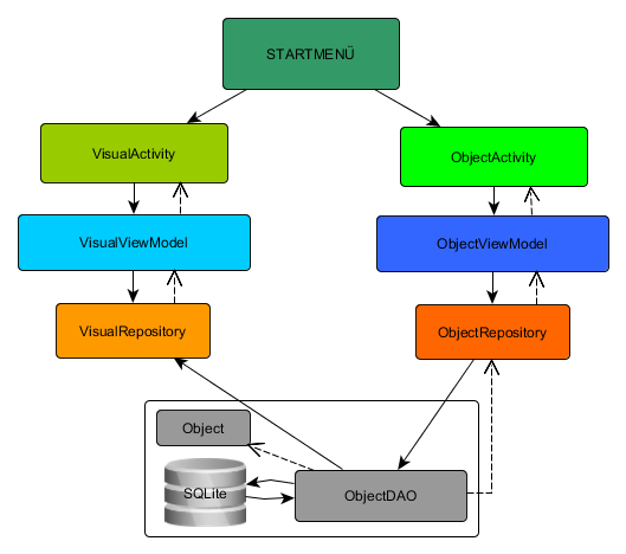
\includegraphics[width=13cm,height=13cm,keepaspectratio]{3Konzeption/Bilder/architektur_konzept.png}
    \caption{Konzeptionelle Software-Architektur}
    \label{pic:architectur}
\end{figure} 

\section{Softwarekonzept}
\label{chap:Softwarekonzept}

\section{Auswahl des AR Frameworks}
\label{chap:Auswahl des AR Frameworks}
Mittlerweile gibt es eine enorme Auswahl an \acs{AR}-Frameworks, die alle unterschiedlich unterschiedliche Präferenzen und 
Einsatzmöglichkeiten haben. Somit sind, auf den Bereich bezogen, Vor- und Nachteile im Vergleich von mehrere Frameworks nicht ausgeschlossen. 
Einige Alternativen wurden getestet und auf deren Brauchbarkeit evaluiert und analysiert. Dazu wurden Kriterien ausgearbeitet, die die 
Auswahl an Frameworks einschränken und nach Möglichkeit das passendste ergeben sollte: 
\begin{enumerate}
    \item Eine performante Darstellung von Objekten.
    \item Möglichkeiten zur Positionsbestimmung.
    \item Eine aktive Community und stetige Weiterentwicklung des Systems.
    \item Möglichkeit zur Integration weiterer Technologien.
    \item Open Source-Projekt, um Flexibilität und weitestgehende Unabhängigkeit zu gewährleisten.
\end{enumerate}
Aufgrund der großen Anzahl an \acs{AR}-Frameworks war es nicht möglich alle in betracht gezogenen Frameworks detailliert aufzuführen, 
lediglich die engere Auswahl der Tools wird aufgegriffen. 
\\ 
Nach ausführlicher Recherche wurden letzten Endes drei Frameworks in die nähere Auswahl aufgenommen, darunter \textit{vuforia}, 
\textit{ARToolkit} und \textit{Google ARCore}. Beweggründe zu dieser Entscheidung war die überwiegende 
Übereinstimmung zu zuvor aufgestellten Kriterien und Anforderungen. Alle Technologien konnten eine aktive und große Community, sowie eine 
aktive Entwicklung, bzw. Weiterentwicklung vorweisen. Zusätzlich bieten alle Frameworks viele Möglichkeiten zur Integration weiterer 
Technologien, um nach Belieben immer mehr Funktionen in das zu entwickelnde System übernehmen zu können. Die Performance der Technologien konnte 
in allen Aspekten überzeugen und ist unter einfachen Bedingungen mehr als ausreichend. Ein Kritikpunkt gegen die Verwendung von vuforia war 
die fehlende Verfügbarkeit des Quellcodes, da dieser unter kostenpflichtiger Lizenz steht und nicht als Open Source-Projekt gilt. Dadurch 
entfiel die Entscheidung für vuforia.
\subsection{ARToolKit}
ARToolKit ist ein \acs{SDK} zur plattformunabhängigen Entwicklung von \acl{AR} Anwendungen. Der Quellcode dieses Frameworks ist seit 2001 
frei verfügbar und ist vielseitig einsetzbar. Das Verfahren zur Positionsbestimmung durch Marker läuft schnell und robust. Marker wie in 
Abbildung \ref{pic:markerARpos} werden schnell und ohne Probleme erkannt. Jedoch gibt es diesbezüglich Einschränkungen die beachtet werden 
müssen, um eine zuverlässige und stabile Markererkennung zu gewährleisten, darunter Verdeckung des Markers, zu große Distanz von Kamera 
zu Marker, Blickwinkel auf den Marker und die Lichtverhältnisse des Umfelds. 
\\ 
Ein gravierender Nachteil des Frameworks für dieses Projekt ist die fehlende Unterstützung der Möglichkeit die 
Umgebung, bzw. das Umfeld zu erkennen und realisieren. So ist das Tracking nur über Marker, bzw. erweiterte 
markerbasierte Tracking-Methoden möglich. 
\\ 
Nach dieser Erkenntnis wurde auch dieses Framework als eher untauglich für die Verwendung in dem Projekt eingestuft. Möglicherweise 
gibt es einen Weg einen \acs{SLAM}-Algorithmus in Kombination mit ARToolKit zu verwenden, allerdings nicht ohne erweiterten Aufwand. 
Somit wurde dieser Weg eingestellt. 
\subsection{Google ARCore}
Google ARCore (siehe Abschnitt \ref{sec:arcore}) konnte bei der Analyse von sich überzeugen. Lediglich die Beschränkung der
Betriebssysteme auf \textit{Android} und \textit{iOS} war ein Nachteil, allerdings nicht von hoher Bedeutung. Der entscheidende Vorteil bei 
ARCore ist der unterstützende Algorithmus zur Umgebungserkennung. Des Weiteren ist Google ARCore ein Open-Source Projekt und befindet sich 
in kontinuierlicher Weiterentwicklung. Neben der stetigen Entwicklung hat sich eine große und aktive Community gebildet, die bei auftauchenden 
Problemen zur Stelle ist. Ein weiterer Vorteil sind die verschiedensten Möglichkeiten der Interaktion mit \acs{AR}-Objekten. Es gibt die 
klassische Markererkennung, die nicht nur mit Markern (siehe Abbildung \ref{pic:markerARpos}) sonder auch mit Bildern funktioniert, dem sogenannten
\textit{AugmentedImage}. Die Erkennung von Gesichtern, \textit{AugmentedFace} und die Erkennung von realen Punkten, Oberflächen und Gegenständen.
\\
\linebreak
Durch diese ganzen positiven Aspekte ist die Wahl des Frameworks auf das von Google entwickelte ARCore gefallen und wurde wegen den überzeugenden 
Grundlagen als Framework für dieses Projekt eingesetzt.

\section{Datenmodell}
\label{chap:Datenmodell}